\documentclass[11pt]{article}
\usepackage[margin=1in]{geometry}
\usepackage[T1]{fontenc}
\usepackage{lmodern}
\usepackage{amsmath,amssymb,amsthm,mathtools}
\usepackage{graphicx,booktabs,tabularx}
\usepackage{microtype}
\usepackage[hidelinks]{hyperref}
\usepackage{fancyhdr}
\pagestyle{fancy}\fancyhf{}
\fancyhead[L]{\small Geometry and readout updates}
\fancyhead[R]{\small Section 3 research note 3}
\fancyfoot[C]{\thepage}
\setlength{\headheight}{14pt}\setlength{\emergencystretch}{2em}
\allowdisplaybreaks
\newtheorem{proposition}{Proposition}[section]
\newcommand{\R}{\mathbb R}
\newcommand{\norm}[1]{\left\lVert#1\right\rVert}
\newcommand{\ip}[2]{\left\langle#1,#2\right\rangle}
\newcommand{\sech}{\operatorname{sech}}
\newcommand{\dd}{\,\mathrm d}
\newcommand{\Eref}{E_{\mathrm{refit}}}
\newcommand{\Ecur}{E_{\mathrm{current}}}
\graphicspath{{figures/}{docs/appendix_notes/2026-09-25-revised/figures/}}
\title{Useful Geometry Motion under Reweighted Training}
\author{Research notes and saved evidence for appendix development}
\date{25 September 2026}

\begin{document}
\maketitle
\begin{abstract}
The useful finding from the geometry experiments is that the baseline updates underuse directions that improve approximation. Increasing the independent slope learning rate works with centers fixed. Amplifying the approximation component of the geometry gradient works from Xavier initialization, and separate Adam streams with the multiplier outside normalization produce much larger improvements. A structured shared-scale Adam control learns geometries whose numerical readout refits reach roughly $10^{-14}$--$10^{-12}$ relative error, although its trained readout remains inaccurate. This note records the settings and quantitative evidence, derives the exact loss split behind the interventions, and connects them to Fourier sensitivity and finite-horizon slope budgets. The results establish useful geometry learning and identify update allocation as a practical issue; they do not by themselves establish the full proposed causal chain from residual refinement to a persistent training barrier.
\end{abstract}

\section{The findings to preserve}

Three interventions changed the geometry outcome substantially. In D25, a larger slope learning rate improved the available approximation even when centers were held fixed. In D29, giving the approximation gradient much more weight improved the refitted geometry on all four Xavier targets. In D31, normalizing the approximation and readout-gap gradients separately with Adam, then weighting the approximation update \emph{after} normalization, produced substantially more accurate geometries at suitable weights. Table~\ref{tab:overview} collects representative endpoints; the comparisons and metrics are specified below.

\begin{table}[htbp]
\centering
\small
\begin{tabularx}{\textwidth}{@{}>{\raggedright\arraybackslash}p{0.23\textwidth}>{\raggedright\arraybackslash}p{0.19\textwidth}>{\raggedright\arraybackslash}X@{}}
\toprule
Intervention & Setting & Saved result \\
\midrule
Larger independent slope rate, D25 & Fixed centers; 2,000 steps &
Mixed-sine refit $0.206\to3.42\times10^{-4}$; Runge $0.0124\to8.43\times10^{-6}$. \\
\addlinespace
Shared-scale Adam, D25 & Fixed uniform centers; 10,000 steps &
All four refits $2.03\times10^{-14}$--$7.79\times10^{-13}$; solved coefficient norms $0.674$--$10.708$. \\
\addlinespace
Weighted profile GD, D29 & Xavier; $\mu=10^5$; 500 steps &
All four refits improve over ordinary GD; Runge $0.1473\to0.01278$. \\
\addlinespace
Split Adam, D31 & Xavier; $\mu=500$; 500 steps &
Mixed sine $3.42\times10^{-7}$, Runge $8.38\times10^{-10}$, Gaussian envelope $1.83\times10^{-5}$. \\
\bottomrule
\end{tabularx}
\caption{Examples of useful geometry learning from the primary reports \cite{D25,D29,D31}. All errors are relative $L_2$ errors after a numerical readout refit, evaluated on independent samples. The first row is initial-to-final improvement along the enhanced-rate run; its original-rate controls barely improve. The D29 row compares terminal controls. Different starts and horizons make this a summary of interventions, not a ranking under one common protocol.}
\label{tab:overview}
\end{table}

\subsection{The common problem and the two error measurements}

The finite-domain experiments use
\begin{equation}
 f_{\theta,v}(x)=d+\sum_{j=1}^{W}c_j\tanh(a_jx+b_j),
 \qquad \theta=(a,b),\quad v=(d,c),\quad
 L=\frac1{2n}\sum_{i=1}^{n}\bigl(f_{\theta,v}(x_i)-g(x_i)\bigr)^2.
 \label{eq:model}
\end{equation}
Here geometry means the feature parameters, and the readout means their output coefficients. The reported scale is $\gamma_j=|a_j|$. When $a_j\ne0$, the corresponding center is $z_j=-b_j/a_j$.

The four targets on $[-1,1]$ are
\begin{align}
 g_{\rm sine}(x)&=\sin(2\pi x), &
 m(x)&=\sin(2\pi x)+\tfrac12\sin(6\pi x)+\tfrac14\sin(14\pi x),\\
 g_{\rm Runge}(x)&=(1+25x^2)^{-1},&
 g_{\rm Gaussian}(x)&=e^{-(x/0.4)^2/2}m(x).
\end{align}
The mixed-sine target is $m$. Training uses $n=1{,}024$ uniform midpoint samples, float64 arithmetic, and full batches. The width convention $N=128$ gives 129 interior neurons plus 24 halo neurons on each side, hence $W=177$. Uniform centers have spacing $h=2/128$. Independent evaluation uses 8,192 different midpoint samples. These are finite-interval problems for \emph{all four} targets, including Gaussian \cite{D25,D29,D31}.

At a saved geometry, a numerical least-squares solve on the training samples produces a diagnostic readout $v_\tau$. Evaluation compares
\begin{equation}
 \Ecur=\frac{\norm{f_{\theta,v}-g}_{\rm eval}}{\norm{g}_{\rm eval}},
 \qquad
 \Eref=\frac{\norm{f_{\theta,v_\tau}-g}_{\rm eval}}{\norm{g}_{\rm eval}}.
 \label{eq:errors}
\end{equation}
The solve retains singular values greater than $10^{-13}$ times the largest. Thus $\Eref$ measures a function available at the learned geometry under a specified numerical solve; $\Ecur$ measures the network actually trained. D25 performs these solves only after training. D29 and D31 also use solved quantities to compute the added geometry gradient, but never install solved coefficients into the trained readout. The large distinction between the two errors is a result of the experiments, not a notation detail.

\section{Why the approximation component is a useful intervention}

\subsection{The exact loss split and its derivative}

Normalize the feature matrix and target by
\begin{equation}
 A_{i0}=n^{-1/2},\qquad A_{ij}=n^{-1/2}\tanh(a_jx_i+b_j),
 \qquad y_i=n^{-1/2}g(x_i).
\end{equation}
Then $r=Av-y$ and $L=\norm{r}^2/2$. Let $A^\dagger$ be the Moore--Penrose pseudoinverse and $P=AA^\dagger$ the orthogonal projector onto the feature span. Define
\begin{equation}
 v_*=A^\dagger y,\qquad
 r_*=Av_*-y=-(I-P)y,\qquad
 F(\theta)=\min_vL(\theta,v)=\tfrac12\norm{r_*}^2.
\end{equation}
The residual is $r=r_*+A(v-v_*)$, and $A^Tr_*=0$. Taking the squared norm therefore gives the exact orthogonal decomposition
\begin{equation}
 \boxed{L(\theta,v)=F(\theta)+G(\theta,v),\qquad
 G(\theta,v)=\tfrac12\norm{A(v-v_*)}^2\geq0.}
 \label{eq:FG}
\end{equation}
$F$ is the best sampled approximation at the current geometry with unrestricted coefficients. $G$ is the unfinished readout-fit gap.

To differentiate $F$, work locally where $A(\theta)$ is continuously differentiable and has constant rank; $v_*$ is then a smooth minimum-norm choice. For a geometry direction $u$, define the fixed-readout Jacobian by
\begin{equation}
 J(v)u=DA(\theta)[u]v,\qquad J_*=J(v_*).
\end{equation}
Differentiating the reduced residual and using the normal equations gives
\begin{align}
 DF[u]
 &=\ip{r_*}{DA[u]v_*+A\,Dv_*[u]}\\
 &=\ip{r_*}{J_*u},\qquad
 \boxed{\nabla F=J_*^Tr_*=[(I-P)J_*]^Tr_*.}
 \label{eq:envelope}
\end{align}
The readout derivative vanishes from the scalar gradient because $A^Tr_*=0$. This is the exact variable-projection envelope identity \cite{handoff,projection}.

Let $h_F=\nabla F$ and $h_G=\nabla_\theta G$. Under ordinary joint flow with geometry rate $\eta_\theta$,
\begin{equation}
 \dot\theta=-\eta_\theta(h_F+h_G)
 \quad\Longrightarrow\quad
 \boxed{\dot F=-\eta_\theta\bigl(\norm{h_F}^2+\ip{h_F}{h_G}\bigr).}
 \label{eq:Fdot}
\end{equation}
The gap gradient can help or oppose approximation improvement. A much larger, mildly opposing $h_G$ can make $F$ increase while the actual loss decreases. Weighting the approximation contribution changes the first term to $-\eta_\theta\mu\norm{h_F}^2$. This identifies a concrete way to give geometry quality more influence; it does not require a claim that the two gradients always cancel.

\subsection{The numerical objective actually used}

The experiments retain a singular subspace $U_\tau$ and use
\begin{equation}
 F_\tau=\tfrac12\norm{(I-U_\tau U_\tau^T)y}^2,\qquad
 G_\tau=L-F_\tau.
 \label{eq:numerical-profile}
\end{equation}
On smooth regions between cutoff crossings, $DF_\tau$ includes motion of this retained subspace. In particular, if $r_\tau=Av_\tau-y$, then
\begin{equation}
 DF_\tau[u]=\ip{r_\tau}{DA[u]v_\tau+A\,Dv_\tau[u]}.
\end{equation}
Unlike exact unrestricted least squares, $A^Tr_\tau$ need not vanish, so the second term cannot simply be discarded. D29 and D31 implement the corresponding corrected derivative and check it against independent differentiation. Hard cutoff crossings may introduce jumps. Also, although $G_\tau=L-F_\tau$ is an exact scalar identity, it need not be nonnegative for arbitrary coefficients using discarded directions \cite{projection,D29,D31}.

One related distinction is worth keeping brief. The current geometry gradient splits as
\begin{equation}
 \nabla_\theta L=
 \underbrace{J(v)^TPr}_{g_{\rm shared}}+
 \underbrace{J(v)^Tr_*}_{g_{\rm outside}}.
\end{equation}
It uses the \emph{current} readout, whereas \eqref{eq:envelope} uses the solved readout. With $K=J(v-v_*)^Tr_*$, linearity of $J$ in $v$ gives
\begin{equation}
 \nabla F=g_{\rm outside}-K,\qquad
 \nabla_\theta G=g_{\rm shared}+K.
\end{equation}
Amplifying $DF_\tau$ is therefore not generally the same as amplifying the current-readout outside-span contribution. This matters when interpreting tiny current-$J$ projection diagnostics; they do not invalidate the successful approximation-gradient interventions.

\section{The interventions and their quantitative outcomes}

\subsection{D25: increase geometry mobility while keeping the readout rule fixed}

D25 fixes the readout GD rate at $0.002$ and changes the geometry update. Raw-geometry rates are $0.002$, $0.2$, and $20$. A more controlled arm fixes the centers and independently trains the slopes in $\tanh(a_j(x-z_j^0))$, comparing slope rates $0.002$ and $20$ for 2,000 steps. Uniform starts have zero readout. From $\gamma=1$, the enhanced-rate trajectories change independent-grid refit error as follows:
\begin{equation}
 \begin{array}{rcl}
 \text{mixed sine:}&0.206&\longrightarrow 3.42\times10^{-4},\\
 \text{Runge:}&0.0124&\longrightarrow 8.43\times10^{-6},\\
 \text{Gaussian envelope:}&0.223&\longrightarrow 0.0390.
 \end{array}
 \label{eq:D25-independent}
\end{equation}
The original-rate controls barely improve. These are useful approximation changes with no center motion and no trained-readout replacement. They directly show that the available geometry gradient can be underused by the baseline step size \cite{D25}.

The strongest structured result ties all slopes to one shared scale and keeps uniform centers fixed. Only the shared-scale optimizer changes from SGD to Adam, both at nominal rate $0.002$; the readout still uses GD at $0.002$. The shared gradient is the \emph{mean} individual centered-scale gradient, so shared-scale SGD has scalar effective rate $0.002/177$. Adam uses the same mean gradient with $(\beta_1,\beta_2)=(0.9,0.999)$ and $\epsilon_A=10^{-8}$. There is no logarithmic parameterization or positivity clipping. After 10,000 steps from $\gamma=1$, the results are:

\begin{table}[htbp]
\centering
\small
\begin{tabular}{@{}lrrrr@{}}
\toprule
Target & Learned $\gamma$ & $\Eref$ & $\norm{v_\tau}$ & $\Ecur$\\
\midrule
Sine & 6.245 & $6.37\times10^{-14}$ & 0.674 & 0.0225\\
Mixed sine & 13.880 & $7.79\times10^{-13}$ & 10.708 & 0.3214\\
Runge & 7.738 & $3.33\times10^{-13}$ & 0.816 & 0.0535\\
Gaussian envelope & 15.496 & $2.03\times10^{-14}$ & 4.148 & 0.2817\\
\bottomrule
\end{tabular}
\caption{D25 shared-scale Adam from $\gamma=1$, with ordinary readout GD throughout \cite{D25}. All refits use the production cutoff and independent samples. No target-specific scale or stopping threshold was supplied.}
\label{tab:D25-adaptive}
\end{table}

This is high-precision \emph{geometry} learning under a strong uniform-center/shared-scale prior. The modest solved coefficient norms are particularly useful: the small refit errors do not require the enormous coefficients found in some Xavier solves. The final trained readouts still leave substantial error. Figure~\ref{fig:D25} shows both outcomes along the same trajectories.

\begin{figure}[p]
\centering
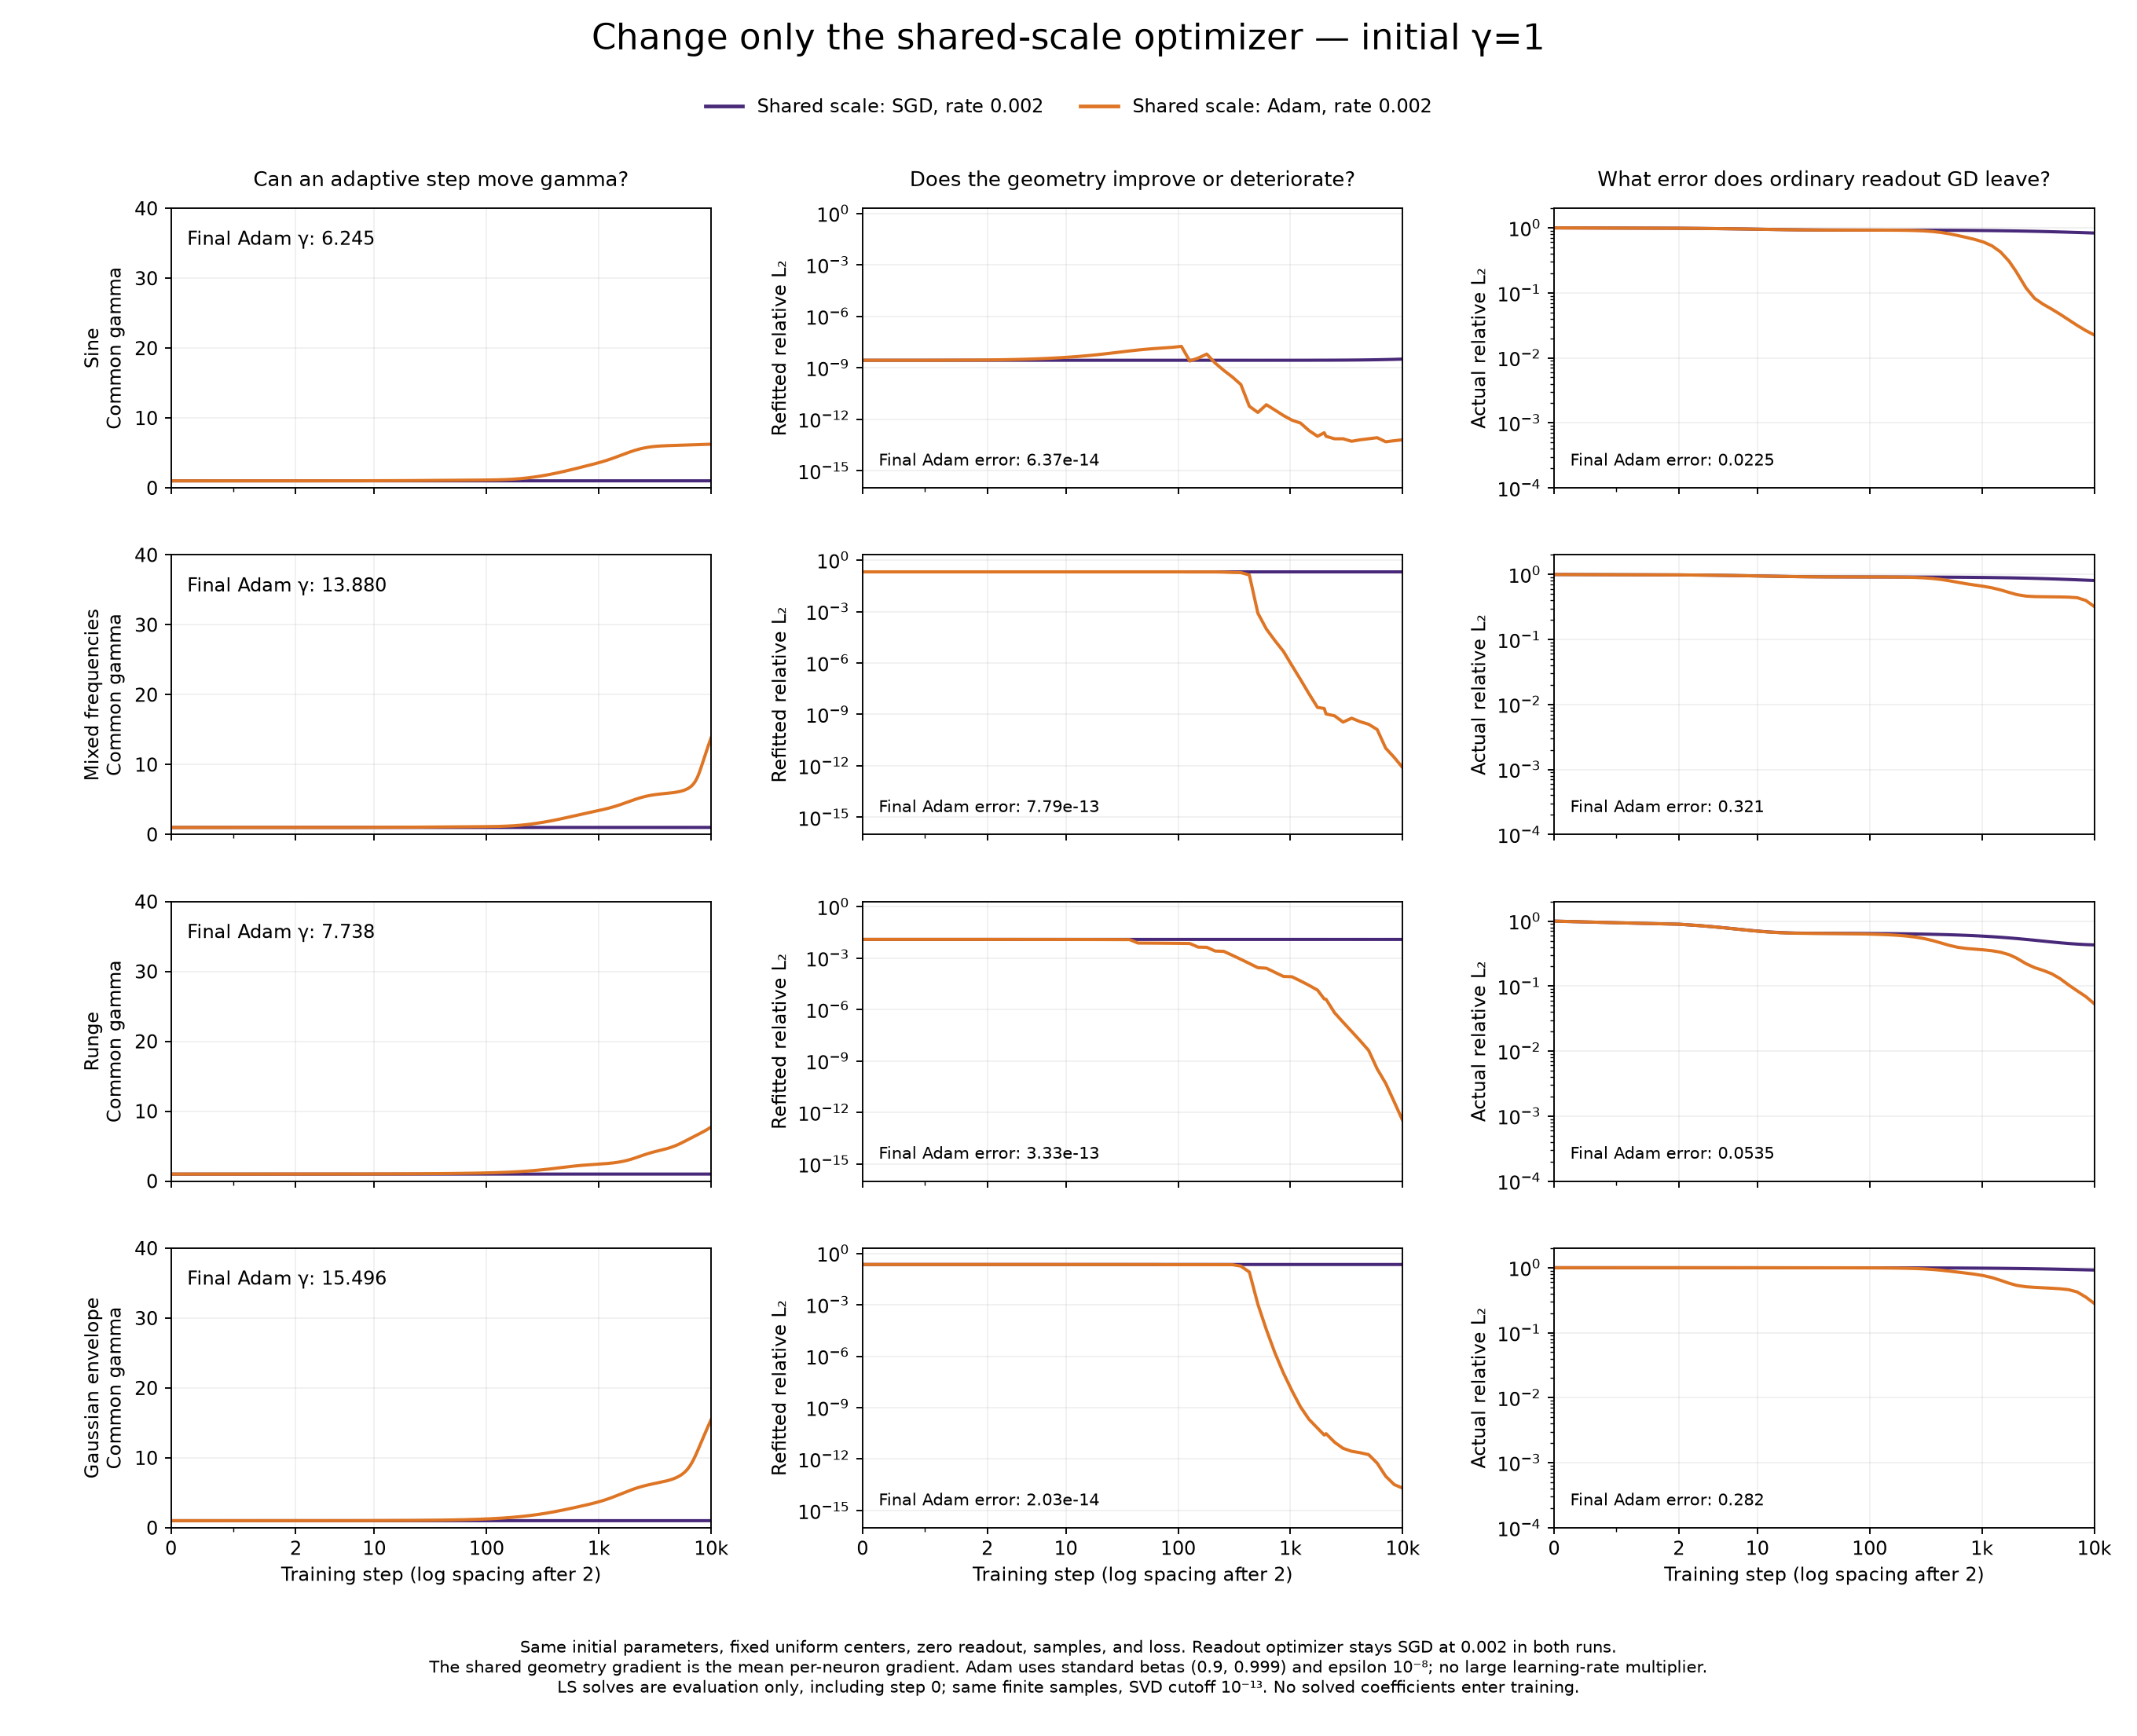
\includegraphics[width=\textwidth]{geometry_adaptive_scale.png}
\caption{D25, reproduced from the saved figure \cite{D25}. Rows are the four targets; columns are shared scale, independent-grid refit error, and current trained-readout error. Orange changes only the shared-scale optimizer to Adam; purple retains shared-scale SGD. Both use nominal geometry rate $0.002$, fixed uniform centers, and readout GD at $0.002$. Adam moves the geometry into a regime with very accurate refits, while readout fitting remains unfinished.}
\label{fig:D25}
\end{figure}

The same intervention starting from already good $\gamma=16$ geometry supplies a useful control. Mixed sine reaches $\gamma=32.605$ with refit error $5.74\times10^{-8}$; Gaussian reaches $\gamma=32.018$ with error $4.55\times10^{-8}$. Both started near numerical precision and improve their \emph{current} fit while losing approximation quality. Thus successful mobility and preservation of a good approximation regime are separate tasks.

\subsection{D29: amplify the approximation gradient}

D29 uses all raw slopes and biases and updates simultaneously by
\begin{equation}
 \theta_{k+1}=\theta_k-\eta\bigl(\mu DF_\tau+DG_\tau\bigr),\qquad
 v_{k+1}=v_k-\eta\nabla_vL,\qquad \eta=0.002.
 \label{eq:weighted-GD}
\end{equation}
Between cutoff crossings this is GD on $H=L+(\mu-1)F_\tau$. It changes the geometry objective while preserving the readout update rule. The full six-weight sweep uses $\mu=1,10,100,10^3,10^4,10^5$. At 500 steps, the largest weight improves the independent-grid refit on every Xavier target:

\begin{table}[htbp]
\centering
\small
\begin{tabular}{@{}lrrr@{}}
\toprule
Target & Ordinary-GD $\Eref$ & $\mu=10^5$ $\Eref$ & Actual loss change\\
\midrule
Sine & 0.005194 & 0.0002067 & $-1.02\%$\\
Mixed sine & 0.4483 & 0.2131 & $+15.57\%$\\
Runge & 0.1473 & 0.01278 & $+14.24\%$\\
Gaussian envelope & 0.4916 & 0.1971 & $-27.18\%$\\
\bottomrule
\end{tabular}
\caption{D29 terminal Xavier comparison at 500 steps \cite{D29}. The actual-loss change is relative to the ordinary-GD control at the same step; negative means improvement.}
\label{tab:D29}
\end{table}

The improvement survives all three tested relative cutoffs, $10^{-12}$, $10^{-13}$, and $10^{-14}$. This larger sweep supersedes the weaker $\mu=1000$ pilot. Geometry gains can coexist with worse actual fitting, exactly as the $F/G$ split permits. The endpoint changes are heterogeneous rather than convergence to uniform $\gamma=16$: at $\mu=10^5$, mean scales are approximately $0.091$, $1.76$, $0.139$, and $0.757$ in target order.

These are real attained-function improvements, but the solved coefficients remain large, approximately $3\times10^8$--$1.4\times10^{10}$. Several audited directions are numerically unresolved. The endpoint evidence is stronger than a claim that these paths accurately integrate the unrestricted exact-profile flow. Each weighted update also performs a dense SVD.

\subsection{D31: separate Adam streams and put the weight outside normalization}

For $Q\in\{F,G\}$, D31 forms $g_k^Q=\nabla_\theta Q_\tau$ at the same state and maintains independent Adam histories:
\begin{align}
 m_k^Q&=\beta_1m_{k-1}^Q+(1-\beta_1)g_k^Q,\qquad
 s_k^Q=\beta_2s_{k-1}^Q+(1-\beta_2)(g_k^Q)^2,\\
 u_k^Q&=\frac{m_k^Q/(1-\beta_1^k)}
 {\sqrt{s_k^Q/(1-\beta_2^k)}+\epsilon_A},\qquad
 \boxed{\theta_{k+1}=\theta_k-\eta_k(\mu u_k^F+u_k^G).}
 \label{eq:split-adam}
\end{align}
All moment operations are coordinatewise. The settings are $\beta_1=0.9$, $\beta_2=0.999$, $\epsilon_A=10^{-8}$, and initial rate $0.002$. The readout uses ordinary Adam on $\nabla_vL$. Geometry remains all raw slopes and biases, with Xavier seed zero \cite{D31}.

The placement of $\mu$ is essential. If an entire stream's input gradients were multiplied by a positive constant, its first moments and square roots of second moments would scale together, largely canceling that factor when $\epsilon_A$ is negligible. Multiplication \emph{after} normalization directly scales the proposed update. Separate histories also make \eqref{eq:split-adam} different from applying one Adam optimizer to $\mu F_\tau+G_\tau$. Even $\mu=1$ does not recover ordinary Adam; the control is a separate ordinary-Adam run on $L$.

The smaller-weight sweep gives markedly better refits than the original $\mu=1000$ choice. Table~\ref{tab:D31} reports two final weights at 500 steps, without selecting an early minimum. At $\mu=500$, Runge's current-model relative error is still $0.0568$, despite its $8.38\times10^{-10}$ refit.

\begin{table}[htbp]
\centering
\small
\begin{tabular}{@{}lrrr@{}}
\toprule
Target & $\mu=100$, 500 steps & $\mu=500$, 500 steps & $\mu=1000$, 500 steps\\
\midrule
Sine & $6.37\times10^{-8}$ & $6.29\times10^{-7}$ & $0.0859$\\
Mixed sine & $0.0492$ & $3.42\times10^{-7}$ & $0.183$\\
Runge & $5.51\times10^{-5}$ & $8.38\times10^{-10}$ & $2.35\times10^{-6}$\\
Gaussian envelope & $0.0223$ & $1.83\times10^{-5}$ & $0.0409$\\
\bottomrule
\end{tabular}
\caption{D31 independent-grid relative refit errors at the final step of the smaller-multiplier sweep \cite{D31}. All settings except the outside multiplier are fixed. Larger weights are not consistently better.}
\label{tab:D31}
\end{table}

The saved 10,000-step extension tests $\mu\in\{50,100,250,500\}$ at constant rate and with cosine decay,
\begin{equation}
 \eta_t=0.002\left[0.001+0.999\frac{1+\cos(\pi t/10000)}2\right],
 \qquad 0\leq t\leq10000.
\end{equation}
The same rate multiplies both geometry streams and the readout step. At the final cosine endpoint, the saved summaries give refits of $1.19\times10^{-10}$ for sine at $\mu=100$, and $3.19\times10^{-7}$, $1.40\times10^{-9}$, and $9.21\times10^{-7}$ for mixed sine, Runge, and Gaussian at $\mu=500$. The corresponding ordinary-Adam refits are $3.46\times10^{-6}$, $0.207$, $0.00590$, and $0.183$. These are selected weights from the saved sweep, not one universally best setting \cite{D31long}.

Runge at $\mu=500$ is a particularly informative long-run endpoint: its solved coefficient norm is about $208$, and its actual error is $0.00265$, compared with ordinary Adam's $0.0202$. The other selected trained-model errors are about $0.0102$, $0.202$, and $0.191$ for sine, mixed sine, and Gaussian. Geometry improvement persists in these examples without closing the readout gap.

\begin{figure}[p]
\centering
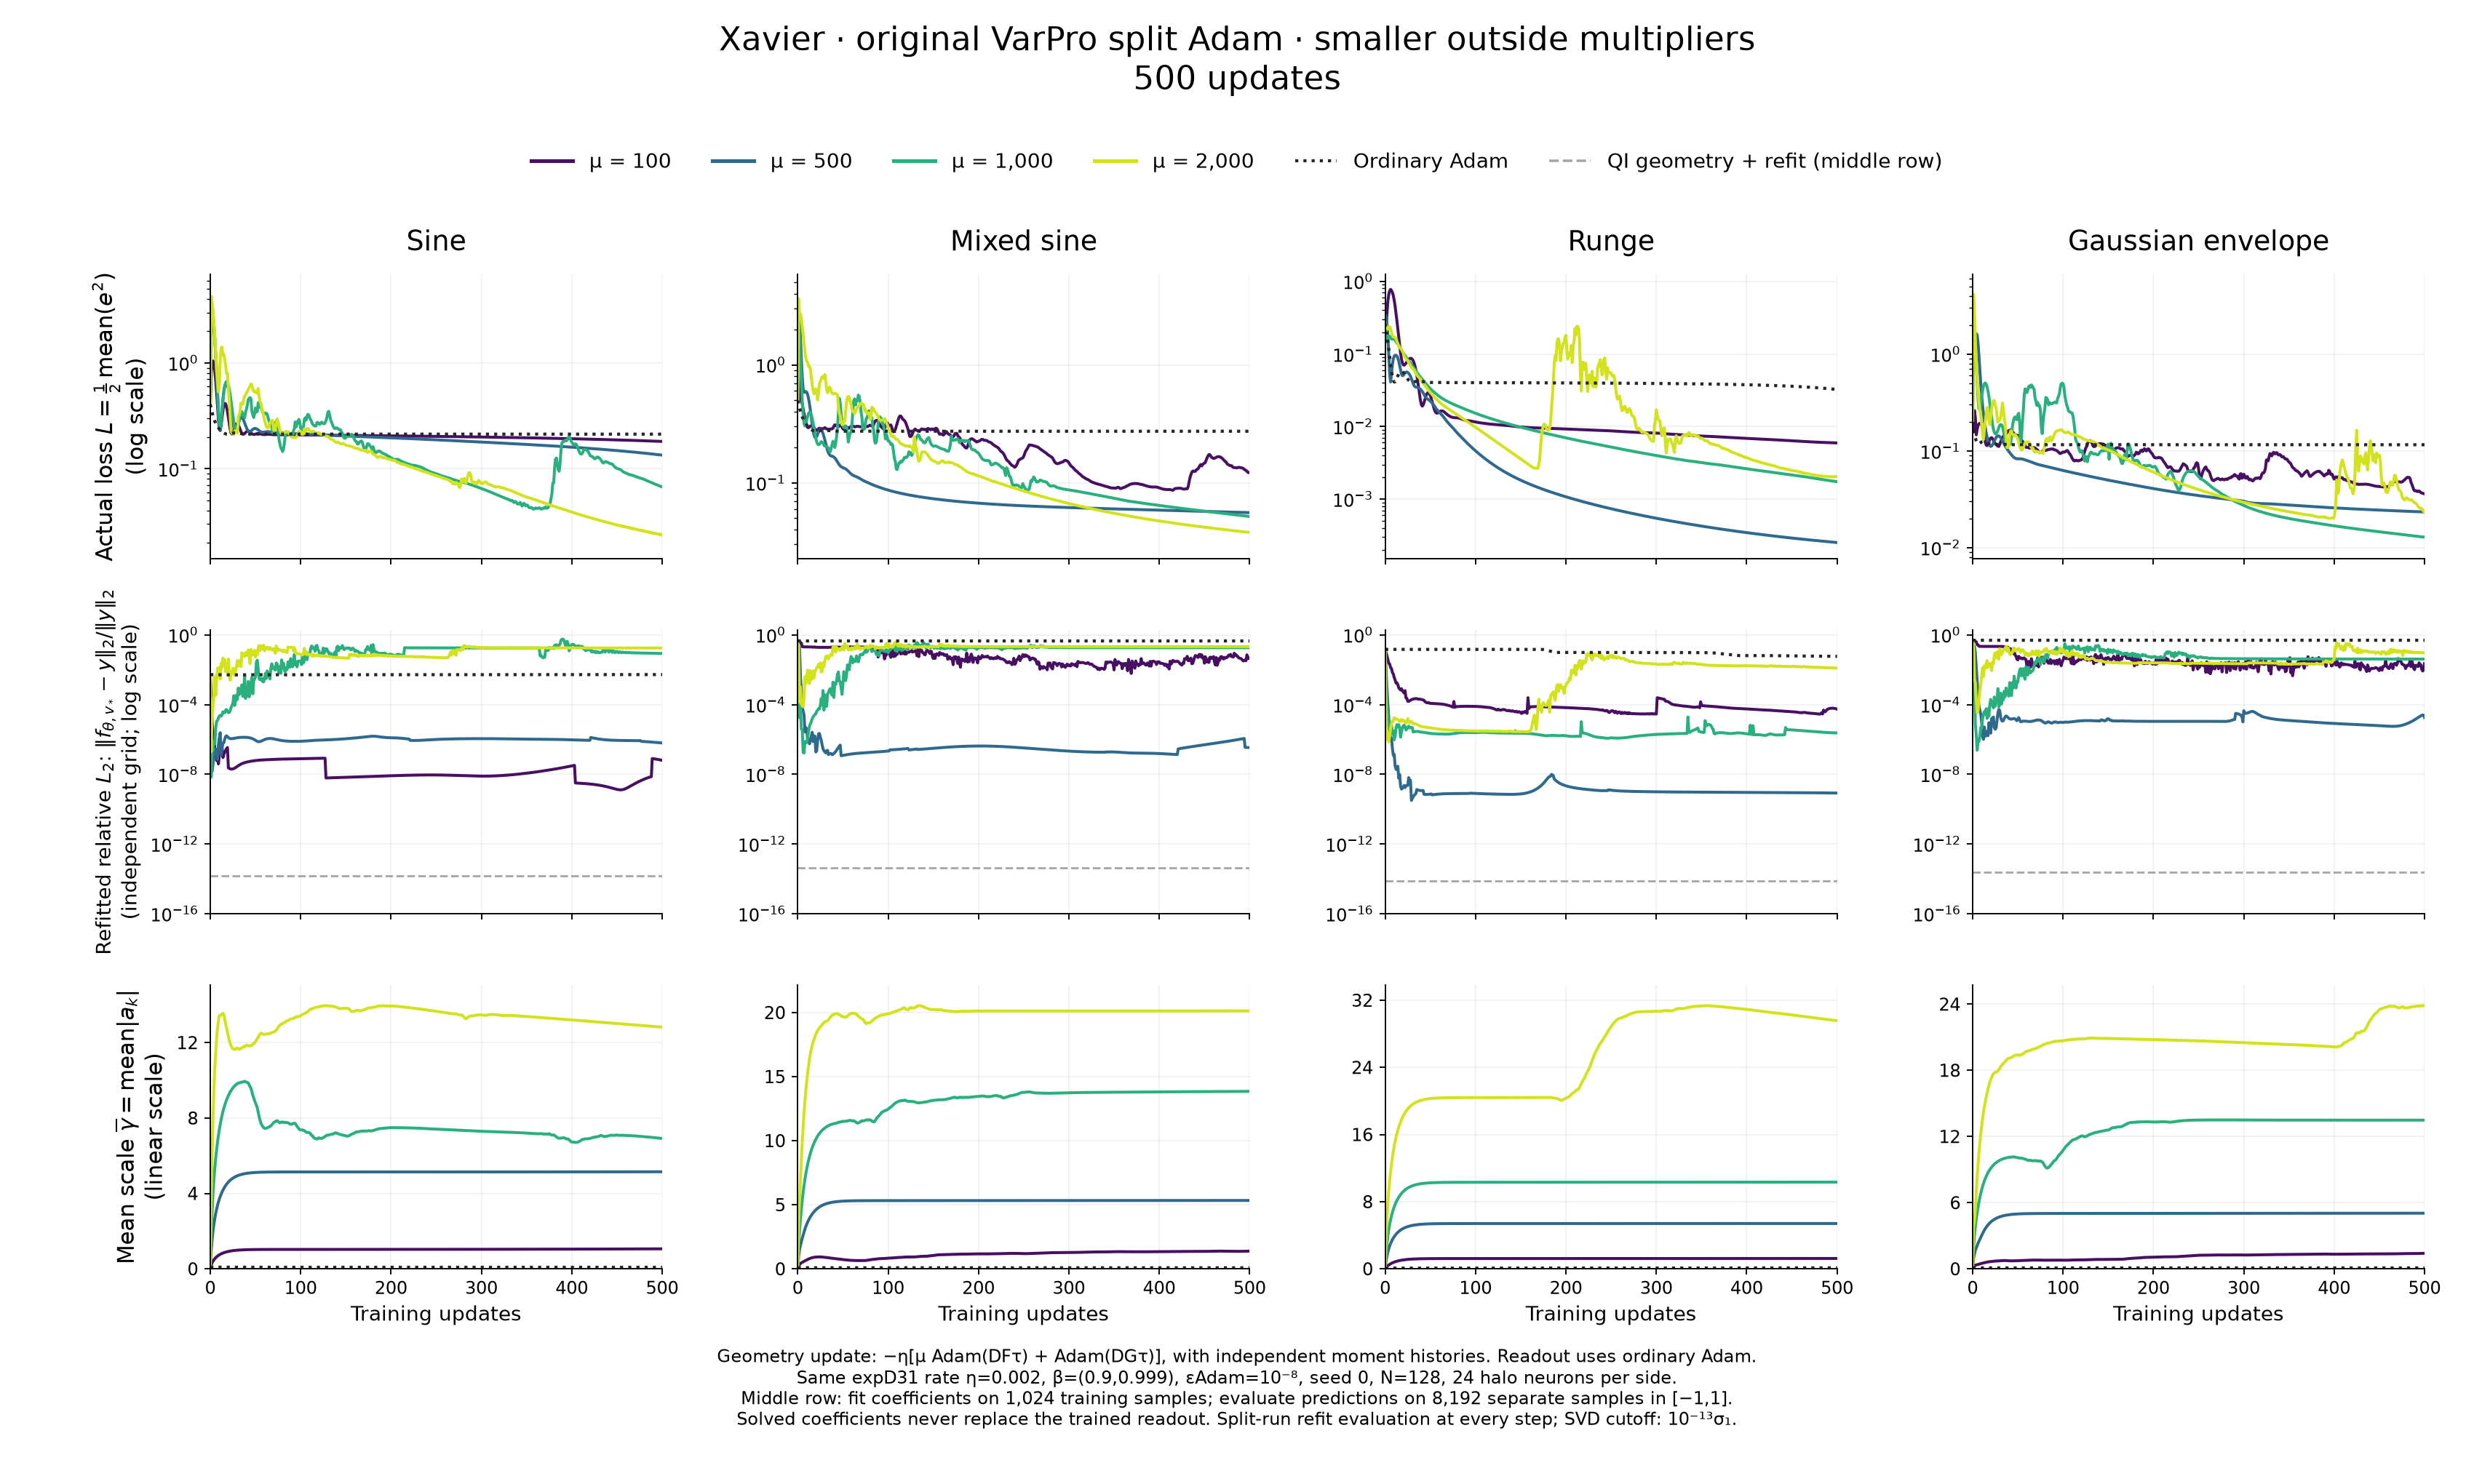
\includegraphics[width=\textwidth]{geometry_split_adam.png}
\caption{D31 smaller outside multipliers, reproduced from the saved figure \cite{D31}. Columns are targets; rows are actual training loss, independent-grid relative refit error, and mean scale. Purple, blue, green, and yellow correspond to $\mu=100,500,1000,2000$. Black dotted curves are ordinary Adam; gray dashed lines mark the QI refit reference. The middle row shows substantial useful geometry learning and why simply increasing the multiplier is insufficient. The top and middle rows measure different outcomes.}
\label{fig:D31}
\end{figure}

The improvement does not make every large step useful. Some trajectories pass through an excellent refitted geometry and later lose it. At Xavier/sine's update-one minimum in the original $\mu=1000$ run, $\norm{DF_\tau}$ is about $1.18\times10^{-12}$, yet the next proposed $F$ displacement has norm about $23.5$ because Adam carries its moment history. At the much larger weight $\mu=10^5$, Runge's sampled refit error is about $0.1$ while independent-grid error is about $413$. These controls identify concrete issues for the method: preserve useful geometry, distinguish sample fit from function fit, and control the magnitude of the normalized update. Initial alternative-backend step discrepancies of roughly $25\%$--$118\%$, one seed, and the SVD at every step limit claims of reproducibility and scalability \cite{D31}. They do not erase the verified attained refit improvements.

\section{Fourier suppression and residual refinement: the supported connection}

\subsection{The scale tangent really suppresses high frequencies}

For this calculation use a centered neuron $c\tanh(\gamma(x-z))$ with $\gamma>0$. Let $e(x)=f(x)-g(x)$ and suppose the whole-line loss $L_{\R}=\frac12\int_{\R}e(x)^2\dd x$ is finite and differentiable under the integral. Holding $c$ and $z$ fixed defines the scale tangent
\begin{equation}
 \psi_{\gamma,z}(x)=(x-z)\sech^2(\gamma(x-z)),\qquad
 \partial_\gamma L_{\R}=c\int_{\R}e(x)\psi_{\gamma,z}(x)\dd x.
\end{equation}
With angular-frequency transform $\widehat u(\omega)=\int u(x)e^{-i\omega x}\dd x$, write
\begin{equation}
 T(\xi)=\frac{\pi\xi}{\sinh(\pi\xi/2)},\qquad T(0)=2.
\end{equation}
The transform of $\sech^2(\gamma x)$ is $\gamma^{-1}T(\omega/\gamma)$. Multiplication by $x$ differentiates that transform, and translation gives
\begin{equation}
 \widehat\psi_{\gamma,z}(\omega)
 =i\gamma^{-2}e^{-i\omega z}T'(\omega/\gamma),\qquad
 \partial_\gamma L_{\R}
 =\frac{c}{2\pi}\int\widehat e(\omega)
           \overline{\widehat\psi_{\gamma,z}(\omega)}\dd\omega.
 \label{eq:fourier-pairing}
\end{equation}
This is a signed, phase-sensitive pairing, not a comparison of spectral magnitudes alone.

For $\xi\geq1$, putting $s=\pi\xi/2$ gives
\begin{equation}
 |T'(\xi)|=\pi\frac{s\coth s-1}{\sinh s}
 \leq C_T\xi e^{-\pi\xi/2},\qquad
 C_T=\frac{\pi^2\coth(\pi/2)}{1-e^{-\pi}}.
\end{equation}
Indeed $s\coth s-1\leq s\coth(\pi/2)$ and
$1/\sinh s\leq2e^{-s}/(1-e^{-\pi})$; symmetry gives the same bound for negative $\xi$.

If $\widehat e\in L^1$, $\widehat e(\omega)=0$ for $|\omega|<\Omega$, and $\Omega\geq\gamma$, define
$M_\Omega=(2\pi)^{-1}\int_{|\omega|\geq\Omega}|\widehat e(\omega)|\dd\omega$.
Taking absolute values in \eqref{eq:fourier-pairing} and using that $q e^{-\pi q/2}$ decreases for $q\geq1$ yields
\begin{equation}
 \boxed{|\partial_\gamma L_{\R}|
 \leq C_T|c|M_\Omega\gamma^{-2}
       \frac{\Omega}{\gamma}e^{-\pi\Omega/(2\gamma)}.}
 \label{eq:fourier-bound}
\end{equation}
This proves instantaneous high-frequency suppression relative to scale \cite{handoff}. A finite-window or sampled loss needs its own boundary, density, and sampling control. Low-frequency leakage matters: if $e=e_{<\Omega}+e_{\geq\Omega}$, the identity
$\int|x-z|\sech^2(\gamma(x-z))\dd x=2\log2/\gamma^2$ gives the additional contribution
$2|c|\log2\,\norm{e_{<\Omega}}_\infty/\gamma^2$. A relatively small low-frequency component can therefore dominate the gradient.

\subsection{What readout fitting removes, and what was observed}

At fixed geometry, unit-rate readout flow has the exact residual equation
\begin{equation}
 \dot r=-AA^Tr,\qquad
 r(t)=(I-P)r(0)+e^{-AA^Tt}Pr(0).
 \label{eq:readout-flow}
\end{equation}
Along a left singular vector of $A$ with singular value $\sigma_j$, represented residual decays as $e^{-\sigma_j^2t}$; discrete GD gives factors $1-\eta_k\sigma_j^2$. Thus readout fitting removes the components to which the current features have strong response first. These directions are singular modes of the finite feature matrix and are not automatically Fourier modes.

The saved D24 analyses supply the complementary frequency evidence \cite{ledger,catalogue}:
\begin{itemize}
\item Signed, coefficient-weighted residual--tangent pairings agree with automatic differentiation. Across the reported panels, $R^2>0.999999999$; using identical samples agrees to floating-point precision.
\item Fixed-residual, fixed-center, fixed-readout probes show weak scale gradients when $\gamma$ is small relative to the carrier frequency. The response rises and then falls at sufficiently large $\gamma$: broadening spectral coverage does not imply monotone growth of total sensitivity.
\item In the examined successful regimes, absolute low-band residual errors fall preferentially. The whole-line Gaussian frequency-learning analysis makes this visible without relying only on a growing high-band fraction.
\item Band-resolved signed gradient pairings retain low-frequency contributions, sometimes dominant even when they carry a minority of the residual energy.
\end{itemize}
The whole-line Gaussian experiments use a tail-cancelling model; they are distinct from the matched finite-domain D25/D29/D31 setting. Earlier cross-target comparisons mixed these objectives. The later matched four-way D24 comparison corrects that mismatch and shows baseline joint GD improving the current fit much more than it improves refitted geometry \cite{catalogue,ledger}.

The useful interpretation is therefore that readout fitting can remove readily expressible, often low-frequency error while small scales respond weakly to higher-frequency residual. The rate and weighting interventions demonstrate that useful geometry signals nevertheless remain and can be used. Establishing that this mechanism causes a persistent barrier along joint tanh training would additionally require a trajectory-wide spectral or directional bound; the observed low-frequency leakage prevents treating the clean gap premise of \eqref{eq:fourier-bound} as already verified. The early-freezing test reinforces this distinction: the tested Xavier freezes did not release useful scale growth \cite{ledger}.

\section{Finite-horizon slope budgets}

The following bounds remain useful even without a persistent Fourier gap. They quantify how much movement ordinary descent can accumulate under explicit assumptions. They also explain why changing geometry rates, the objective, or the parameter metric can change the outcome.

\subsection{A direct residual budget in raw coordinates}

For the raw model \eqref{eq:model}, suppose $|x_i|\leq X$ and set $R=\norm{r}$. Cauchy--Schwarz and $\sech^2\leq1$ give
\begin{equation}
 \left|\partial_{a_j}L\right|
 =\left|\frac{c_j}{n}\sum_i(f(x_i)-g(x_i))x_i\sech^2(a_jx_i+b_j)\right|
 \leq X|c_j|R.
\end{equation}
Thus unit-rate raw-geometry flow and simultaneous GD with geometry step $\eta_k$ obey
\begin{equation}
 |a_j(T)-a_j(0)|\leq X\int_0^T|c_j|R\dd t,\qquad
 |a_{j,K}-a_{j,0}|\leq X\sum_{k<K}\eta_k|c_{j,k}|R_k.
 \label{eq:direct-budget}
\end{equation}
The reverse triangle inequality gives the same displacement bounds for $\gamma_j=|a_j|$. Joint center and readout motion do not invalidate the calculation; their effects enter the actual $c_j$ and residual trajectory. For a fixed-center slope derivative, replace $X$ by a bound on $|x_i-z_j|$.

For example, if $|c_j|\leq C$ and $R(t)\leq B e^{-\nu t}+R_{\rm floor}$ with $\nu>0$, then
\begin{equation}
 |a_j(T)-a_j(0)|\leq XC\left[\frac{B}{\nu}(1-e^{-\nu T})+TR_{\rm floor}\right].
\end{equation}
The actual residual and coefficient magnitudes, not an evaluation-only refit floor, determine this bound. It has not yet been turned into a measured practical escape-time certificate for the intervention runs \cite{ledger}.

\subsection{The energy proof, without a coefficient bound}

\begin{proposition}[Continuous finite-horizon budget]
Let $p$ contain all trainable raw parameters and let $a$ be its slope subvector. Suppose a nonnegative differentiable objective $\mathcal L$ and a solution of ordinary Euclidean gradient flow $\dot p=-\nabla\mathcal L(p)$ are defined on $[0,T]$, with the chain rule and integrals below valid. Then
\begin{equation}
 \norm{a(T)-a(0)}^2
 \leq\left(\int_0^T\norm{\dot a}\dd t\right)^2
 \leq T\bigl(\mathcal L(p(0))-\mathcal L(p(T))\bigr)
 \leq T\mathcal L(p(0)).
 \label{eq:energy-flow}
\end{equation}
\end{proposition}
\begin{proof}
The chain rule gives $\frac{\dd}{\dd t}\mathcal L(p(t))=-\norm{\nabla\mathcal L(p(t))}^2=-\norm{\dot p(t)}^2$. Integration yields
\begin{equation}
 \int_0^T\norm{\dot p(t)}^2\dd t=\mathcal L(p(0))-\mathcal L(p(T)).
\end{equation}
The endpoint displacement is at most the slope path length. Cauchy--Schwarz bounds its square by
$T\int_0^T\norm{\dot a(t)}^2\dd t$, which is no greater than
$T\int_0^T\norm{\dot p(t)}^2\dd t$. Nonnegativity gives the final inequality.
\end{proof}

\begin{proposition}[Discrete finite-horizon budget]
Suppose $p_{k+1}=p_k-\eta_k\nabla\mathcal L(p_k)$, where $\eta_k>0$, $\mathcal L_k\geq0$, and every step satisfies the sufficient-descent inequality
\begin{equation}
 \mathcal L_k-\mathcal L_{k+1}
 \geq\alpha\eta_k\norm{\nabla\mathcal L(p_k)}^2
 \quad\text{for one fixed }\alpha>0.
 \label{eq:descent}
\end{equation}
Writing $S_K=\sum_{k<K}\eta_k$, one has
\begin{equation}
 \norm{a_K-a_0}^2
 \leq\left(\sum_{k<K}\norm{a_{k+1}-a_k}\right)^2
 \leq\frac{S_K}{\alpha}(\mathcal L_0-\mathcal L_K)
 \leq\frac{S_K\mathcal L_0}{\alpha}.
 \label{eq:energy-GD}
\end{equation}
\end{proposition}
\begin{proof}
The slope path length is $\sum_{k<K}\eta_k\norm{\nabla_a\mathcal L(p_k)}$. Weighted Cauchy--Schwarz and \eqref{eq:descent} give
\begin{align}
 \left(\sum_{k<K}\eta_k\norm{\nabla_a\mathcal L(p_k)}\right)^2
 &\leq S_K\sum_{k<K}\eta_k\norm{\nabla_a\mathcal L(p_k)}^2\\
 &\leq\frac{S_K}{\alpha}\sum_{k<K}(\mathcal L_k-\mathcal L_{k+1})
 =\frac{S_K}{\alpha}(\mathcal L_0-\mathcal L_K).
\end{align}
\end{proof}

For example, if the gradient is $\beta$-Lipschitz on every update segment and $\eta_k\leq1/\beta$, the descent lemma gives
\begin{equation}
 \mathcal L_{k+1}\leq\mathcal L_k
 -\eta_k(1-\beta\eta_k/2)\norm{\nabla\mathcal L(p_k)}^2,
\end{equation}
so $\alpha=1/2$ is valid. The full tanh/readout objective does not automatically have a global uniform $\beta$, and observed monotone loss alone does not supply a uniform positive $\alpha$ \cite{energy}.

If the target slope set is at Euclidean distance at least $D$ from initialization and $\mathcal L_0>0$, reaching it requires
\begin{equation}
 T\geq\frac{D^2}{\mathcal L_0},\qquad
 S_K\geq\frac{\alpha D^2}{\mathcal L_0};
 \qquad K\geq\frac{\alpha D^2}{\eta\mathcal L_0}
 \ \text{at constant }\eta.
\end{equation}
The same proof can restart after fitting has already reduced the loss. Over a future horizon $H$ from $t_f$, it gives
\begin{equation}
 \norm{a(t_f+H)-a(t_f)}^2\leq H\mathcal L(t_f).
 \label{eq:remaining}
\end{equation}
This is a precise finite-budget sense in which a smaller remaining objective limits further raw movement. For joint GD, $\mathcal L$ is the actual training loss $L$, not $F_\tau$. For exact weighted-profile GD it is the weighted objective; for true profiled flow it is the profiled objective. The clocks and loss budgets must match the algorithm being discussed.

\subsection{Width and learning-rate consequences}

Suppose every initial slope obeys $|a_j(0)|\leq g_0<\Gamma$, and a specified target set requires at least $M$ slopes with magnitude at least $\Gamma$. Any endpoint in that set satisfies
\begin{equation}
 D^2\geq M(\Gamma-g_0)^2,
\end{equation}
because each of those coordinates has moved by at least $\Gamma-g_0$, regardless of sign changes. The subset can be selected at the endpoint because the initial bound is uniform. A mean initial scale cannot replace this premise.

If $\Gamma=\lambda_*/h=\Theta(W)$, $g_0=O(1)$, $\mathcal L_0=O(1)$, and $M=\Theta(W)$, the necessary continuous time is $\Omega(W^3)$; the necessary discrete accumulated rate has that order if $\alpha$ stays bounded below. Requiring one such slope gives $\Omega(W^2)$. These statements concern reaching that set. Using them as an accuracy theorem would require a separate argument that every admissible accurate representation needs such movement.

A block learning-rate change changes the metric. For a constant positive diagonal matrix $D_p$ and flow $\dot p=-D_p\nabla\mathcal L$,
\begin{equation}
 \int_0^T\norm{\dot p}_{D_p^{-1}}^2\dd t=\mathcal L_0-\mathcal L_T,
 \qquad
 \norm{p(T)-p(0)}_{D_p^{-1}}^2\leq T(\mathcal L_0-\mathcal L_T).
\end{equation}
Larger slope rates reduce the metric cost of slope motion; this is compatible with D25's success. A tied scale pays one scalar distance, while log-scale descent pays distance in $\log\gamma$. D31's separate Adam histories and outside multiplier do not satisfy the ordinary Euclidean-GD hypotheses automatically.

Finally, these bounds neither prove instability of faster schemes nor permanent nonreachability. For the scalar quadratic $\mathcal L(p)=\beta p^2/2$, the stable step $\eta=1.9/\beta$ has descent coefficient $0.05$, not $1/2$. Also, finite integrated squared speed permits an unbounded path over infinite time: \eqref{eq:energy-flow} grows like $\sqrt T$ in distance. The useful conclusion is a conditional finite-horizon restriction \cite{energy}.

\section{The research conclusion supported by these materials}

There is a usable geometry signal in the tested finite-domain problems. Larger slope rates exploit it without center motion; approximation-gradient weighting exploits it from Xavier; and split normalization with outside weighting can improve refitted accuracy by many orders of magnitude. The structured shared-scale control reaches a particularly strong approximation regime with modest solved coefficients. These are the positive findings to carry into an appendix discussion.

The mathematical picture explains why ordinary training can spend most of its progress on the current readout fit, why residual refinement can leave weak scale response, and why a finite remaining loss budget limits raw motion. The still-open issue is how to preserve and use the learned approximation while fitting the readout accurately, with reliable directions and acceptable cost. The saved results support that narrower, concrete research problem more strongly than either an assertion that geometry cannot learn or a claim that the full persistent Fourier-depletion mechanism has already been proved.

\begin{thebibliography}{9}
\small
\bibitem{D25}
Project report, \emph{expD25: Separating scale mobility, geometry quality, and readout fitting}. Primary settings and endpoint tables.\\
\path{results/checkpoint_D_optimizers/expD25_scale_barrier/expD25_results.md}\\
Copied figure: \path{figures/adaptive_gamma_1.png} within that experiment's results directory.

\bibitem{D29}
Project report, \emph{expD29: Sweep the approximation-gradient weight}. Uses the completed six-weight sweep, rather than only the initial $\mu=1000$ pilot.\\
\path{results/checkpoint_D_optimizers/expD29_weighted_profile/expD29_results.md}

\bibitem{D31}
Project report, \emph{expD31: Separate Adam streams with an outside approximation multiplier}. Primary update definition, smaller-weight sweep, and numerical checks.\\
\path{results/checkpoint_D_optimizers/expD31_split_adam/expD31_results.md}\\
Copied figure: \path{mu_refit_sweep/figures/xavier.png} within that experiment's results directory.

\bibitem{D31long}
D31 saved long-run endpoint and validation summary. Values in this note are read from existing saved summaries; no trajectory or refit was recomputed.\\
\path{results/checkpoint_D_optimizers/expD31_split_adam/long_run/data/summary.json}

\bibitem{ledger}
Project evidence ledger, 19 September 2026, especially Sections 1, 2, 5, and 6.\\
\path{docs/scale_mismatch_evidence_ledger.md}

\bibitem{catalogue}
Project session catalogue, including the training-domain correction and the D24 matched four-way comparison.\\
\path{docs/expD24_session_catalogue.md}

\bibitem{handoff}
\emph{The $\gamma$-barrier: Residuals, projections, and bounds on scale drift}, revision 2, 8 September 2026, Sections 2, 3, and 5. Source of the Fourier and raw-drift derivations retained here.\\
\path{docs/appendix_materials/2026-09-25/sources/attachments/gamma_barrier_handoff_v2.pdf}

\bibitem{projection}
Project projection audit and theoretical framework. Sources for the exact profile/current-readout distinction and the joint-flow derivative of $F$.\\
\path{docs/gamma_barrier_synthesis/projection_audit.md}\\
\path{docs/gamma_barrier_synthesis/theory_framework.md}

\bibitem{energy}
Project energy-bound audit. Source of the continuous/discrete finite-horizon budgets and their metric and stability qualifications.\\
\path{docs/gamma_barrier_synthesis/energy_bound_audit.md}
\end{thebibliography}

\end{document}
